\section{Caminho máximo em árvores}
\label{sec:caminhoMaximo}
	Um dos passos do algoritmo FST é a determinação 
	de um caminho máximo em uma árvore.
	Encontrar um caminho máximo em uma árvore~${T=(V,E)}$ é uma 
	tarefa computacionalmente simples que pode ser realizada em 
	tempo~$O(n)$, sendo~$n$ o número de vértices de~$T$, ou 
	seja,~${n =|V|}$. 

	Primeiramente escolhe-se um vértice arbitrário~$v \in V$ e 
	encontra-se um vértice~$y_0$ mais distante de~$v$ em~$T$.
	Depois, repetimos o mesmo processo a partir de~$y_0$, 
	encontrando um vértice~$x_0$ mais distante de~$y_0$ em~$T$.

	Para encontrar um vértice mais distante de algum vértice dado, 
	basta usar uma busca em largura em~$T$.  
	Feito isso, como demonstraremos a seguir,
	temos um caminho máximo em~$T$: o~$x_0,y_0\caminho$.

	\bigskip

	\begin{lem}
	\label{lema:caminhoMax}
		O~$x_0,y_0\caminho$ é um caminho máximo em~$T$.
	\end{lem}

	\bigskip

	\begin{proof}
		Suponha que exista um outro caminho mais longo que 
		o~$x_0,y_0\caminho$ e sejam~$x$ e~$y$ os seus extremos.

	        \textbf{Caso 1:} O~$x,y\caminho$ e 
	        o~$x_0,y_0\caminho$ não possuem vértices em comum.

	        Existe um~$a,b\caminho$ em~$T$, de 
	        comprimento~$c \ge 1$, que conecta os dois caminhos, 
	        com apenas o vértice~$a$ 
	        no ~$x,y\caminho$ e apenas o vértice~$b$ 
	        no~$x_0,y_0\caminho$.

	        \begin{center} 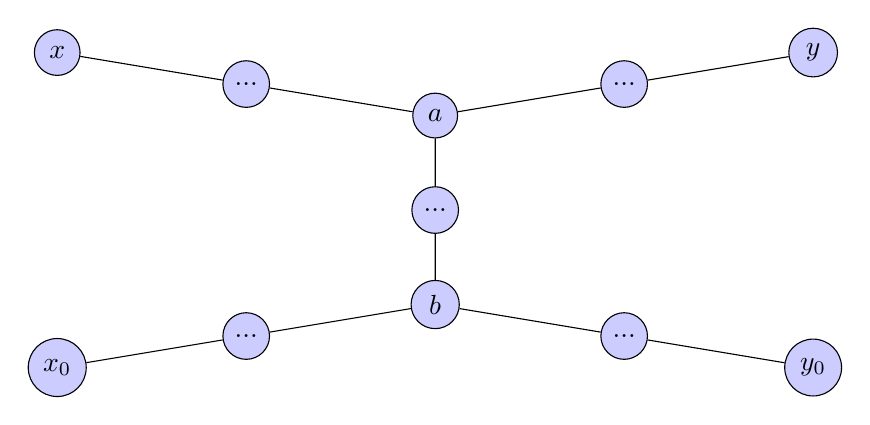
\begin{tikzpicture}
				[scale=.8,auto=left,every node/.style={circle, 
				draw=black,
				fill=blue!20}]
				\node (x) at (0,5)  {$x$};
				\node (y) at (12,5) {$y$};
				\node (a) at (6,4)  {$a$};
				  
				\node (x0) at (0,0) {$x_0$};
				\node (y0) at (12,0) {$y_0$};
				\node (b)  at (6,1)  {$b$};

				\node (n1) at (3,4.5) {...}; %entre x e a 
				\node (n2) at (9,4.5) {...}; %entre a e y
				\node (n3) at (3,0.5) {...}; %entre x0 e b
				\node (n4) at (9,0.5) {...}; %entre y0 e b
				\node (n5) at (6,2.5) {...}; %entre a e b

				\foreach \from/\to in {x/n1,n1/a,a/n2,n2/y,x0/n3,
				n3/b,b/n4,n4/y0,a/n5,b/n5}
				\draw (\from) -- (\to);
			\end{tikzpicture} \end{center}


	        Como estamos em uma 
	        árvore,~${\dist(x,y) =\dist(x,a)+\dist(a,y)}$
	        e~${\dist(x_0,y_0) =\dist(x_0,b)+\dist(b,y_0)}$.
	        Como o~$x,y\caminho$ é 
	        máximo,~${\dist(x,y)\ge \dist(x_0,y)}$,
	        e isso implica que~${\dist(x,a)\ge \dist(x_0,b)+c}$.
 			
 			Temos que~${\dist(x_0,y_0)\ge \dist(x,y_0)}$,
	        pois~$x_0$ é um vértice mais distante de~$y_0$ e isso implica 
	        que~${\dist(x_0,b)\ge \dist(x,a)+c}$.
	        Logo temos 
	        que~${\dist(x,a)\ge \dist(x, a)+2c}$,
	        uma contradição, visto que~${c\ge 1}$.


			\bigskip
			\bigskip
			\bigskip


			\textbf{Caso 2:} O~$x,y\caminho$ e 
			o~$x_0,y_0\caminho$ possuem vértices em comum.

			A interseção entre esses dois caminhos é 
			um~$a,b\caminho$ de comprimento~$c \ge 0$.
			Podemos assumir, sem perda de generalidade, 
			que~${\dist(x,a) \le \dist(x,b)}$ e 
			que~${\dist(x_0,a) \le \dist(x_0,b)}$, como na figura 
			abaixo.
			(Do contrário troque~$a$ por~$b$ e possivelmente~$x$
			por~$y$.)

			\begin{center} 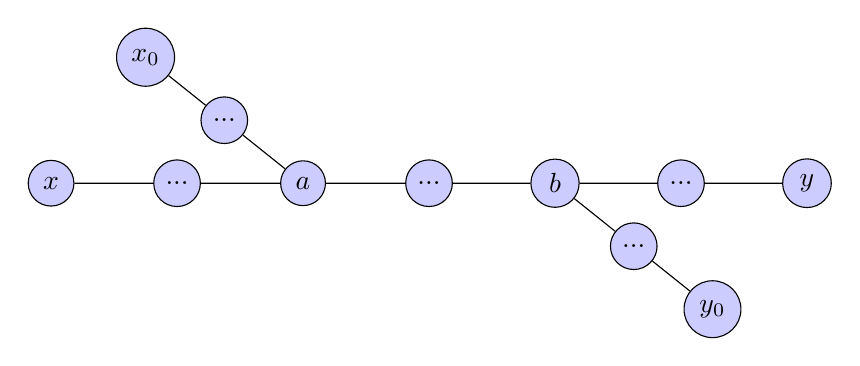
\begin{tikzpicture}
				[scale=.8,auto=left,every node/.style={circle, 
				draw=black,
				fill=blue!20}]
				\node (x) at (0,4)  {$x$};
				\node (y) at (12,4) {$y$};
				\node (a) at (4,4)  {$a$};
				\node (b) at (8,4)  {$b$};
				\node (x0) at (1.5,6)  {$x_0$};
				\node (y0) at (10.5,2)  {$y_0$};
				  
				\node (n1) at (2,4) {...};
				\node (n2) at (6,4) {...};
				\node (n3) at (10,4) {...};
				\node (n4) at (9.25,3) {...};
				\node (n5) at (2.75,5) {...};

				\foreach \from/\to in {x/n1,n1/a,a/n2,n2/b,b/n3,
				n3/y, a/n5,n5/x0,b/n4,n4/y0}
				\draw (\from) -- (\to);
			\end{tikzpicture} \end{center}


			Temos que~${\dist(x_0,a)\ge \dist(x,a)}$,
			pois~$x_0$ é um vértice mais distante de~$y_0$.
			Por outro lado, como~$x$ é um vértice mais distante
			de~$y$, temos também que~${\dist(x,a)\ge \dist(x_0,a)}$
			e, portanto,~${\dist(x_0,a) =\dist(x,a)}$.
			Similarmente, como~$y$ é um vértice mais distante 
			de~$x$, vale que~${\dist(y,b) \ge \dist(y_0,b)}$.

			Agora consideremos o vértice~$v$ que foi escolhido 
			arbitrariamente no início do algoritmo, e seja~$v'$
			o vértice mais próximo de~$v$ no~$x_0,y_0\caminho$.
			%Se~$v'\ne b$, então, 
			Como~$y_0$ é um vértice mais 
			distante de~$v$,
			\begin{align}
				\dist(v',y_0) &\ge \dist(v',y) =\dist(v',b) + 
				\dist(b,y)\nonumber \\
				&\ge \dist(v',b) + \dist(b,y_0) \ge \dist(v',y_0) 
				\nonumber,
			\end{align} 
			o que implica que~${\dist(v',y_0)~=\dist(v',y)}$ 
			e~${\dist(b,y)~=\dist(b,y_0)}$. 
			Ou seja,~${\dist(x,y) =\dist(x_0,y_0)}$,
			% Resta analisar o caso em que~$v'=b$ (é um caso 
			% especial, dado que pode-se ter arestas em comum 
			% entre o~$v,v'\caminho$ e o~$y,b\caminho$).
			% Como~$y$ é um vértice mais distante de~$x$, temos 
			% que~$\dist(v',y_0) \le \dist(v',y)$.
			% Como~$x_0$ é um vértice mais distante de~$y_0$, temos
			% que~$\dist(x_0,v') \ge \dist(y,v')$.
			% Finalmente, como~$y_0$ é um vértice mais distante 
			% de~$v$, vale que~$\dist(y_0,v')\ge \dist(x_0,v')$.
			% Dessas três desigualdades, concluímos 
			% que~${\dist(y_0,v')=\dist(y,v')=\dist(x_0,v')=\dist(x,v')}$,
			% onde a última igualdade vale pois já mostramos 
			% que~${\dist(x_0,a) =\dist(x,a)}$.
			% Assim sendo,~${\dist(x_0,y_0) =\dist(x,y)}$, 
			completando a prova.
	\end{proof}

	\bigskip
	\bigskip


%%%%%%%%%%%%%%%%%%%%%%%%%%%%%%%%%%%%%%%%%%%%%%%%%%%%%%%%%%%%%%%%%%%

